\section{第三章 \quad 流体动力学基础}

%\subsection{描述流体运动的两种方法}

\pt{流场}:充满运动流体的质点的全部空间

\pt{拉格朗日法}:跟踪个别流体质点的运动历程,研究其位移、速度、加速度随时间的变化;综合考察全部流体质点；得到整个流场的运动规律。数学上求解困难,实际较为少用\\
\pt{欧拉法}:分析流场中每一空间点上的流体质点运动，进而研究整个流体的运动规律。着眼于整个流场状态，也称局部法或流场法。选定空间固定点；研究流体质点经过该点时速度、压强、密度等的变化；把许多空间点在不同时刻的运动情况记录下来；得到流场规律。

\m{
    \left\{
    \begin{aligned}
         & u = u(x,y,z,t)        \\
         & v=v(x,y,z,t)          \\
         & w=w(x,y,z,t)          \\
         & p=p(x,y,z,t)          \\
         & \rho = \rho (x,y,z,t)
    \end{aligned}
    \right.
    \left\{
    \begin{aligned}
         & a_x = \frac{\partial u}{\partial t}+u \frac{\partial u}{\partial x} + v \frac{\partial u}{\partial y}+w \frac{\partial u}{\partial z} \\
         & a_y = \frac{\partial v}{\partial t}+u \frac{\partial v}{\partial x}+v \frac{\partial v}{\partial y}+w \frac{\partial v}{\partial z}   \\
         & a_z = \frac{\partial w}{\partial t}+u \frac{\partial w}{\partial x}+v \frac{\partial w}{\partial y}+w \frac{\partial w}{\partial z}
    \end{aligned}
    \right.
}

可写成 \m{\vec{a}= \frac{\mathrm{d}V}{\mathrm{d}t} = \underbrace{\frac{\partial V}{\partial t}}_{\text{当地加速度}}+\underbrace{(\vec{V}\cdot \nabla)\vec{V}}_{\text{迁移加速度}}}

%\subsection{流体运动的基本概念}

\divider

\m{\frac{\partial }{\partial t}=0} 时为定常流动,与时间无关;\m{v\cdot \nabla = 0}时为均匀流动\\

\pt{迹线}是流场中某一流体质点的运动轨迹，是同一流体质点在不同时刻形成的曲线。为\pt{拉格朗日法}的研究内容\\
微分方程为 \m{\frac{\mathrm{d}x}{u}=\frac{\mathrm{d}y}{v}=\frac{\mathrm{d}z}{w}=\mathrm{d}t}\\
\pt{流线}是某一瞬时在流场中作的一条曲线，曲线上各流体质点的速度方向都与该曲线相切。是同一时刻不同流体质点组成的曲线，属于\pt{欧拉法}的研究内容。流线密集处流速大，流线稀疏处流速小\\
微分方程为\m{\frac{\mathrm{d}x}{u(x,y,z,t)}=\frac{\mathrm{d}y}{v(x,y,z,t)}=\frac{\mathrm{d}z}{w(x,y,z,t)}}\\
\pt{流管}为由流线组成的管状曲面,表面的流体速度与管表面相切,没有流体质点穿过流管表面\\
\pt{流束}为过流管横截面上各点作流线，得到充满流管的一束流线簇。流管指外轮廓，流束指内部\\
\pt{微元流束}：横截面积很小的流束；当流束横截面积趋近于零时，流束达到极限，即流线\\
流束是物理概念，涉及流速、压强、动量、能量、流量等；流线是数学概念，只是某一瞬时流场中的一条光滑曲线。\\
\pt{有效截面}：流束中与各流线相垂直的横截面，也称过流断面。\\
\pt{总流}：截面积有限大的流束。\\
\pt{有压流动}：总流的全部边界受固体边界约束，流体充满流道，如压力水管中的流动。\\
\pt{无压流动}：总流边界一部分受固体边界约束，另一部分与气体接触并形成自由液面，如明渠中的流动。\\
\pt{射流}：总流全部边界均无固体边界约束，如喷嘴出口的流动。\\
\pt{体积流量}：\m{q_\mathrm{v}=\iint_A \vec{V}\cdot \mathrm{d}\vec{A}}\\
\pt{质量流量}：\m{q_\mathrm{m}=\iint_A \rho\vec{V} \cdot \mathrm{d}\vec{A}}

\divider

%\subsection{流体流动的连续性方程}

\pt{质量体}：流场中封闭流体面所包含的流体，也成为闭系统。边界随流体一起运动，形状和大小可随时间变化，边界面上没有质量交换，边界面上与外界可以有力的相互作用和能量交换。对应拉格朗日方法\\
\pt{控制体}：被流体流过的、由相对于某一坐标系不随时间变化的封闭曲面包含的流体，也成为开系统。几何外形和体积相对于选定坐标系不变，控制面上可以有质量交换，流体与外界可以有力的相互作用和能量交换。对应欧拉方法\\
\pt{流体运动的连续性条件}：流体连续地充满所占据空间，流动时内部不形成空隙。来源于质量守恒定律\\
可压缩流体非定常三维连续性方程：\m{\frac{\partial\rho}{\partial t}+\frac{\partial(\rho u)}{\partial x}+\frac{\partial(\rho v)}{\partial y}+\frac{\partial(\rho w)}{\partial z}=0}\\
可压缩流体定常三维连续性方程为 \m{\frac{\partial(\rho u)}{\partial x}+\frac{\partial(\rho v)}{\partial y}+\frac{\partial(\rho w)}{\partial z}=0}\\
可压缩流体定常三维连续性方程为 \m{\frac{\partial(\rho u)}{\partial x}+\frac{\partial(\rho v)}{\partial y}+\frac{\partial(\rho w)}{\partial z}=0}\\
不可压缩流体三维连续性方程为 \m{\frac{\partial u}{\partial x}+\frac{\partial v}{\partial y}+\frac{\partial w}{\partial z}=0}\\
不可压缩流体二维连续性方程为 \m{\frac{\partial u}{\partial x}+\frac{\partial v}{\partial y}=0}\\
微元流束的连续性方程为 \m{\rho_1V_1\mathrm{d}A_1=\rho_2V_2\mathrm{d}A_2=\rho V\mathrm{d}A=\mathrm{const}}
总流流动的连续性方程为 \m{\iint_{A_1}\rho_1V_1\,\mathrm{d}A_1=\iint_{A_2}\rho_2V_2\,\mathrm{d}A_2=\iint_A\rho V\,\mathrm{d}A=\mathrm{const}},或 \m{\rho_1\bar{V}_1A+A_1 = \rho_2\bar{V}_2A_2}

\divider

%\subsection{流体运动微分方程}

\pt{理想流体的运动微分方程}/\pt{欧拉运动方程}:\m{\left\{
    \begin{aligned}
         & f_x-\frac{1}{\rho}\frac{\partial p}{\partial x}=\frac{\mathrm{D}u}{\mathrm{D}t} \\
         & f_y-\frac{1}{\rho}\frac{\partial p}{\partial y}=\frac{\mathrm{D}v}{\mathrm{D}t} \\
         & f_z-\frac{1}{\rho}\frac{\partial p}{\partial z}=\frac{\mathrm{D}w}{\mathrm{D}t}
    \end{aligned}
    \right.
}

其中 \m{\frac{\mathrm{D}}{\mathrm{D}t}=\frac{\partial }{\partial t}+u \frac{\partial }{\partial x}+v \frac{\partial }{\partial y}+w \frac{\partial }{\partial z}}。可写成 \m{\vec{f}-\frac{1}{\rho}\nabla p =\frac{\mathrm{D}\vec{V}}{\mathrm{D}t}}

\pt{纳维-斯托克斯方程 Navier-Stokers}

\m{\left\{
    \begin{aligned}
        f_x-\frac{1}{\rho}+\frac{\mu}{\rho}\left(\frac{\partial^2 u}{\partial x^2}+\frac{\partial^2 u}{\partial y^2}+\frac{\partial^2 u}{\partial z^2}\right) & = \frac{\mathrm{D}u}{\mathrm{D}t} \\
        f_y-\frac{1}{\rho}+\frac{\mu}{\rho}\left(\frac{\partial^2 v}{\partial x^2}+\frac{\partial^2 v}{\partial y^2}+\frac{\partial^2 v}{\partial z^2}\right) & = \frac{\mathrm{D}v}{\mathrm{D}t} \\
        f_z-\frac{1}{\rho}+\frac{\mu}{\rho}\left(\frac{\partial^2 w}{\partial x^2}+\frac{\partial^2 w}{\partial y^2}+\frac{\partial^2 w}{\partial z^2}\right) & = \frac{\mathrm{D}w}{\mathrm{D}t}
    \end{aligned}
    \right.
}

考虑黏性的 N-S 方程 \m{\vec{f}-\frac{1}{\rho}+\frac{\mu}{\rho}\delta^2\vec{V}+\frac{1}{3}\frac{\mu}{\rho}\nabla(\nabla\cdot\vec{V})=\frac{\mathrm{D}\vec{V}}{\mathrm{D}t}}\\
无粘流动\m{\vec{f}-\frac{1}{\rho}\nabla p=\frac{\mathrm{D}\vec{V}}{\mathrm{D}t}} 欧拉运动方程\\
静止\m{\vec{f}-\frac{1}{\rho}\nabla p=0} 欧拉静平衡方程

\divider

%\subsection{理想流体微元流束的伯努利方程}

\pt{理想微元流束的伯努利方程}\m{z+\frac{p}{\rho g}+\frac{V^2}{2g}=\mathrm{const}}。使用条件为理想流体、不可压缩均质流体、质量力只有重力、一维定常流动、同一流线或微元流束。

\divider

%\subsection{黏性流体总流的伯努利方程}

\pt{黏性流体微元流束的伯努利方程}\\\m{z_1+\frac{p_1}{\rho g}+\frac{{V_1}^2}{2g}=z_2+\frac{p_2}{\rho g}+\frac{{V_2}^2}{2g}+h_w'}

\pt{均匀流}：同一条流线上各空间点\pt{流速相同}（包括大小方向），过水断面是平面，断面形状与尺寸沿流程不变，断面上压强分布满足静压分布规律 \m{z+\frac{p}{\rho g}=C}；\pt{非均匀流}：流场中同一条流线各空间上的\pt{流速不相同}\\
\pt{缓变流}：流束内流线的夹角很小、流线的曲率半径很大，近乎平行直线的流动有效截面近似为平面，压强分布可按 \m{z+\frac{p}{\rho g}=C} 处理。与之相对的是\pt{急变流}。\pt{非均匀流}在直管内的流动为\pt{缓变流}，在管道内截面积变化剧烈，流动方向发生改变的地方为\pt{急变流}

\pt{黏性流体总流的伯努利方程}\\
\m{z_1+\frac{p_1}{\rho g}+\alpha_1\frac{\bar V_1^2}{2g}=z_2+\frac{p_2}{\rho g}+\alpha_2\frac{\bar V_2^2}{2g}+h_w}\\
\pt{动能修正系数}\m{\alpha=\frac{1}{A}\iint_A\left(\frac{V}{\bar{V}}\right)^3\mathrm{d}A\approx 1\sim 2}，取决于断面流速分布。\pt{平均能量损失}\m{h_w=\frac{1}{q_v}\int_{q_v}h_w\,\mathrm{d}q_v}。$\bar V$ 是有效截面上的平均流速，可按照平均流速理解。\\
方程适用于定常流动、黏性流体、均质不可压缩、质量力只有重力、沿总流满足连续性方程 $q_v=\mathrm{const}$、方程两端过流断面必须是缓变流截面，但两截面之间允许有急变流。\\
\pt{几何意义}：理想流体总水头线为水平线；实际流体总水头线恒为下降曲线；静水头线可升、可降、可水平；均匀流中总水头线平行于静水头线；两线距离为速度水头

\divider

%\subsection{伯努利原理的应用}

\pt{弧线球、香蕉球}与伯努利原理、马格努斯效应有关；旋转造成周围流速分布不同，从而产生压强差。\pt{乒乓球}在气流中不易飞走的演示，体现高速流区压强较低的伯努利效应。\pt{新能源发电}应用：风电叶片翼型设计、能量转换与贝茨极限、风电场尾流效应管理、风速测量与风资源评估。\pt{航空航天}应用：机翼上表面气流速度较大、压强较低，下表面压强较高，形成升力；课件也提醒实际升力还与机翼攻角使气流向下偏转有关。\pt{汽车设计}应用：流线型外形减少车头车尾高压区、降低风阻；尾翼与扰流板用于增加下压力。

\divider

\noindent
\begin{minipage}
    [t]{0.64\linewidth}
    \vspace{0pt}
    \raggedright
    \pt{皮托管测速计}\\
    A 点为驻点，速度为 $0$，压强 $p_A$ 称全压；\\
    B 点速度为 $V$，压强 $p_B$ 称静压。\\
    满足 $\Delta h = \frac{V^2}{2g}$\\
    带修正的 $V=\psi \sqrt{2g\Delta h}$\\
    $\psi\approx 0.97\sim0.99$，一般由实验测定
\end{minipage}
\hfill
\begin{minipage}
    [t]{0.35\linewidth}
    \vspace{0pt}
    \centering
    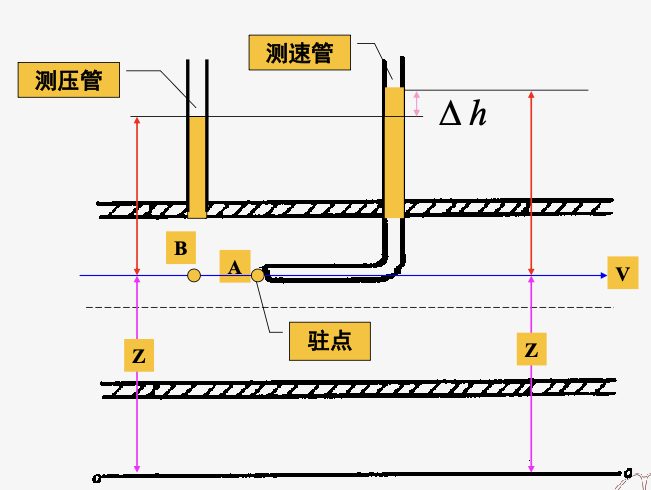
\includegraphics[width=\linewidth]{figures/3皮托管测速计.png}
\end{minipage}

\divider

\noindent
\begin{minipage}
    [t]{0.64\linewidth}
    \vspace{0pt}
    \raggedright
    \pt{文丘里流量计}\\
    以文丘里管水平轴线为基准面，对截面 $1$、$2$ 列伯努利方程：$\frac{p_1}{\rho g}+\frac{V_1^2}{2g}=\frac{p_2}{\rho g}+\frac{V_2^2}{2g}$\\
    由一维流动连续性方程 $V_1=\frac{A_2}{A_1}V_2$,$V_2=\sqrt{\frac{2(p_1-p_2)}{\rho[1-(A_2/A_1)^2]}}$
\end{minipage}
\hfill
\begin{minipage}
    [t]{0.35\linewidth}
    \vspace{0pt}
    \centering
    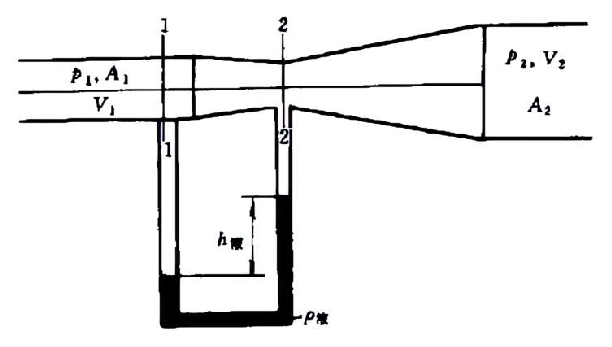
\includegraphics[width=\linewidth]{figures/3文丘里流量计.png}
\end{minipage}

$q_V=A_2V_2=\frac{\pi d_2^2}{4}\sqrt{\frac{2g(\rho_{\mathrm{液}}-\rho)h_{\mathrm{液}}}{\rho[1-(A_2/A_1)^2]}}$，实际体积流量 $q_{V,\mathrm{实}}=C_d q_V$，其中 $C_d$ 为流量系数，通过实验测定

\divider

%\subsection{定常流动的动量方程}

\pt{不可压缩流体动量方程}$\sum\vec{F}=\rho q_V(\beta_2\vec{V}_2-\beta_1\vec{V}_1)$

\divider
